\chapter{Related work}



\section{Visualization tools}
In the following section we will describe existing visualization tools for poetry. There is no specific software for analyzing song lyrics in particular since they can be considered just a more structurally relaxed version of a regular poem.
\subsection{Poem Viewer}
The most complex and comprehensive visualization tool is Poem Viewer \cite{Abdul2013}. With no need for complicated installations it is easily available for the writers as a web-based application as shown in Figure \ref{screenshotPV}. Unfortunately, at the time of writing this thesis the upload of custom text was not working. Luckily, this is still an ongoing project so this might be just a temporary issue. Nevertheless there are some default poems available to demonstrate this software's capabilities.
\begin{figure}[h]\centering
	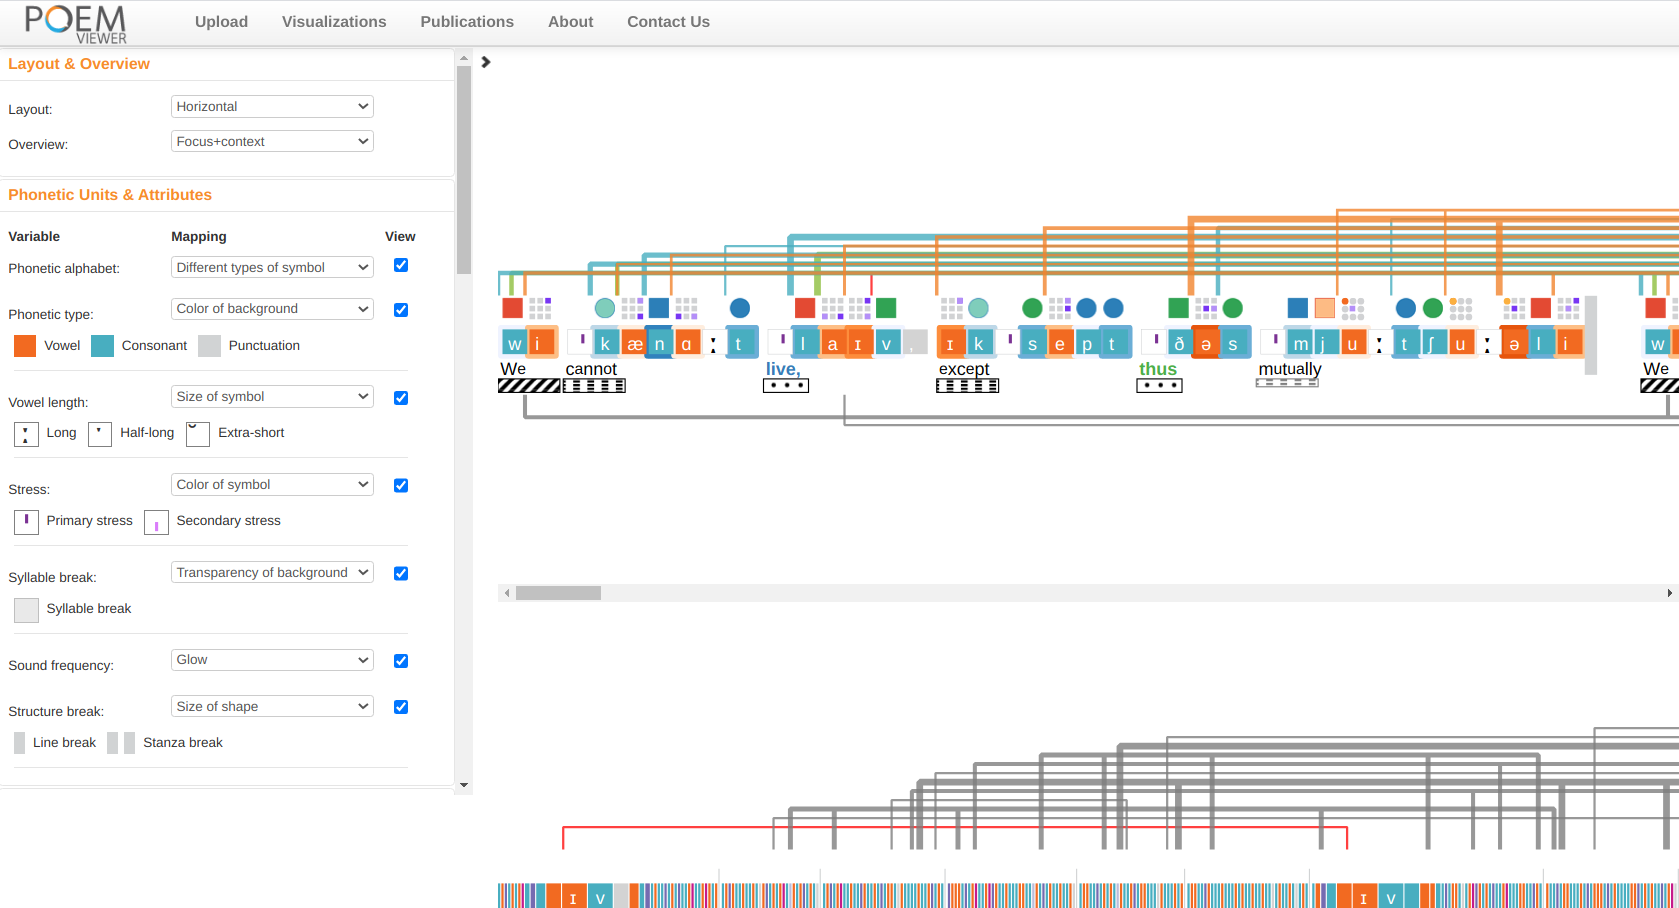
\includegraphics[scale=0.24]{../img/ScreenshotPV.png}
	\caption{Screenshot from Poem Viewer tool - visualizing Love by Elizabeth Barrett Browning.}\label{screenshotPV}
\end{figure}

\begin{figure}[h]\centering
	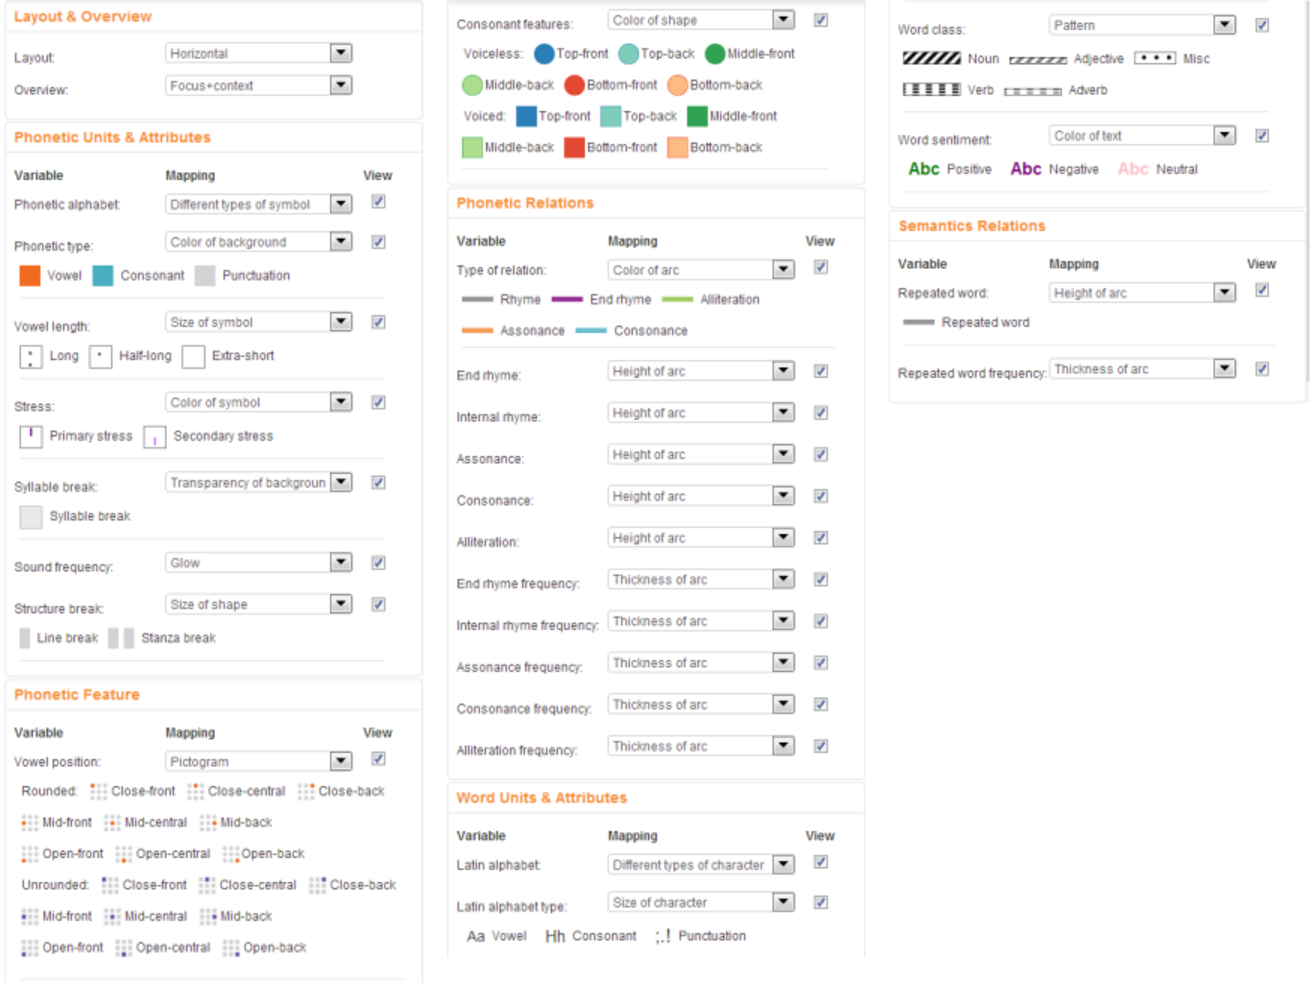
\includegraphics[scale=0.4]{../img/snapshotPV_options.pdf}
	\caption{Available options and their default mappings in Poem Viewer.}\label{screenshotPV-options}
\end{figure}

Most of the analyzed features (shown in Figure \ref{screenshotPV-options} focuses on the phonetic aspects of the poem. After phonetic transcription to IPA users can analyze consonant features, vowel length and position, stress, syllables, word classes and sentiment using color codes and markers. A second layout offers six different graphs/animations of tongue positions during each verse. Arcs are used to mark end rhyme, alliteration, assonance, consonance, their particular frequencies and repeating words.


Overall this software, although very elaborate, appears crowded and confusing for an inexperienced user. It is perhaps better suited for its original use case - a well structured poem - than less regular song lyrics.

\subsection{SPARSAR}
SPARSAR (\cite{Delmonte2014}) is also a very interesting tool for poetry analysis and expressive Text-to-speech conversion. It is originally designed for a thorough examination of a very strictly structured Shakespeare's sonnets. To achieve this, it has to run analyses on many levels - and these results can be used to analyze any poem. It looks at the poem on three views: phonetic (pronunciation, consonant and vowel tongue position, assonances, etc.), poetic (metrical structure, rhyme schemes, acoustic length, etc.), and semantic (sentiment, methaphorically linked words, anaphora, etc.).

User can choose between a window application with graphs and diagrams or a headless mode with .xml output files. Its main disadvantage for our usecase is that it's written in Prolog and therefore is very strict on the input format and runs only under a specific older version of Ubuntu. \todo[inline]{Should I mention here that I used it or save it for later chapters?}

\subsection{ProseVis}
This Java desktop visualization tool by \cite{Clement2013} analyzes text through
parts-of-speech, accent, phoneme, stress, tone, and break index. These features are extracted using OpenMary Text-to-speech system (\cite{Schroder2006}) and predictive classification. The authors believe their visualization will present the features to user in a more human readable form \footnote{https://sourceforge.net/projects/prosevis/}.

\begin{figure}[h]\centering
	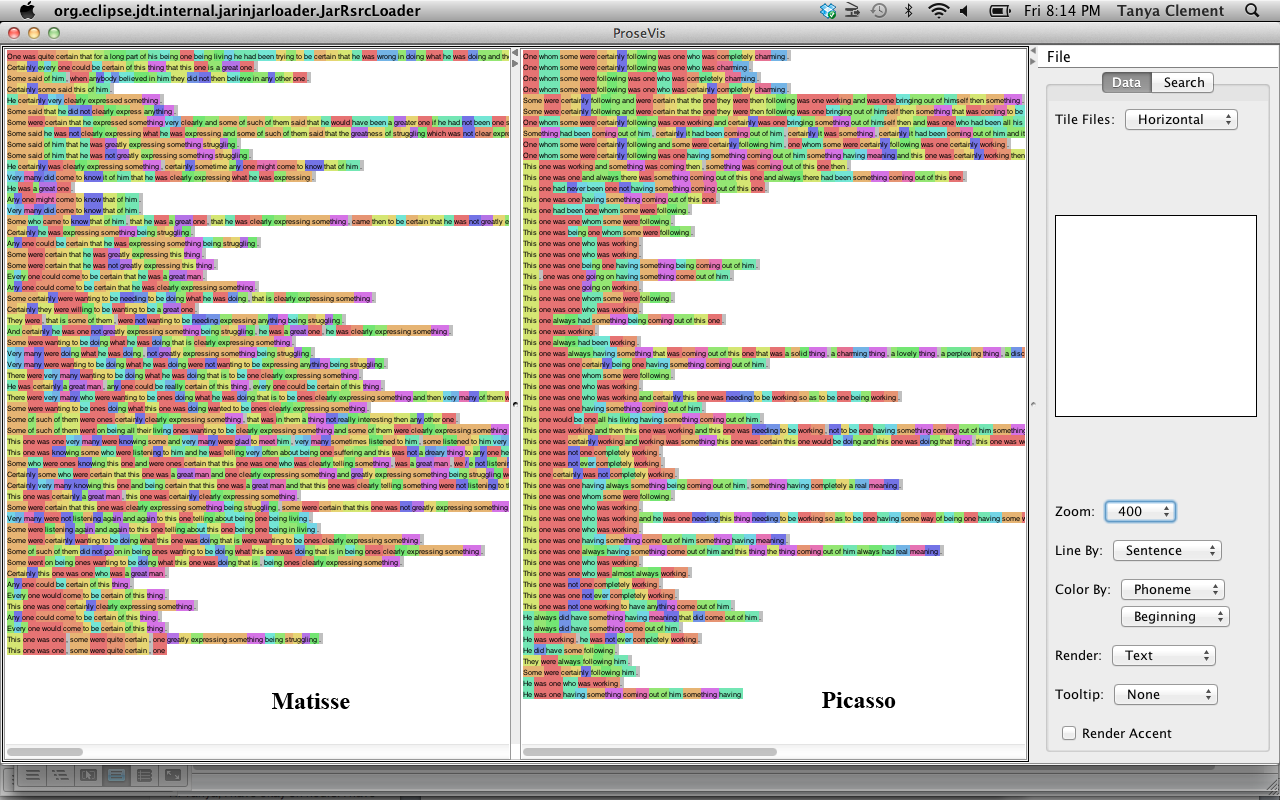
\includegraphics[scale=0.24]{../img/prosevis.png}
	\caption{Comparison of two poems in ProseVis.}\label{screenshotProsevis}
\end{figure}

\subsection{RhymeDesign}
RhymeDesign is an open-source MacOS application for analysis of sonic devices in poetry \cite{McCurdy2015}. User can enter their poem and query for one of the default rhyme types or choose a custom rhyme type.
\subsection{Ambiances}
This software is unique in the fact that it the analysis is integrated in the process of writing. As described in the paper \cite{Meneses2015}, writers enter the poem, receive a visualization and can control this visualization with body and hand gestures which in turn influence the poem. However we were not able to find the actual program.


\section{Generation tools}
